\chapter{Grundeinstellungen TIA-Portal}\label{chap:Grundeinstellungen TIA-Portal}

\section{Sprachen}\label{subsec:Sprachen}
Die Sprache muss sowohl in der PLC-Programmierung als auch im HMI immer konsistent sein. Das heißt, dass keinesfalls Sprachen in einem Projekt gemischt werden dürfen (z.B. Englisch als Editiersprache und deutsche Kommentare in Bausteinen oder französische Texte im englischen Sprachbereich des HMIs). \par
\noindent Wenn nicht ausdrücklich vom Kunden anders gewünscht, ist die Sprache „English (United States)“ als Editier- und Referenzsprache für die PLC-Programmierung zu verwenden. Somit werden auch der Programmcode und alle Kommentare in Englisch verfasst. Nur falls der Kunde eine anderssprachige Software explizit bestellt, ist die Software in der geforderten Sprache zu schreiben und für diesen Fall die Editiersprache entsprechend einzustellen. Die Benutzeroberfläche ist entsprechend Landessprache bzw. Kundenwunsch zu erstellen. 

\begin{figure}[!ht]
    \centering
    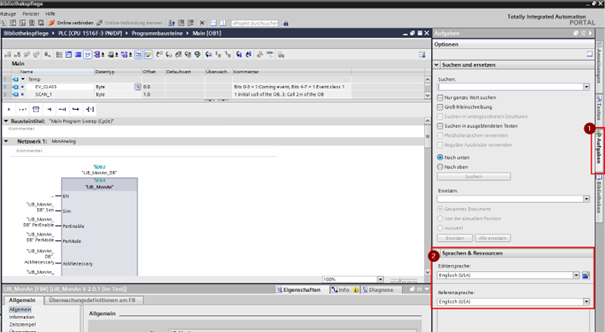
\includegraphics[width = 0.8 \textwidth]{Einstellungen der Referenz- und Editiersprache.png}
    \caption{Einstellungen der Referenz- und Editiersprache}
    \label{fig:Einstellungen der Referenz- und Editiersprache}
\end{figure}

\clearpage

\section{Mnemonik}\label{subsec:Mnemonik}

Die Spracheinstellung für Programmiersprachen ist entsprechend der Software auf International einzustellen, es sei denn, der Kunde bestellt dies ausdrücklich anders. Die folgenden Bilder zeigen, wo diese Einstellung vorzunehmen ist.

\begin{figure}[!ht]
    \centering
    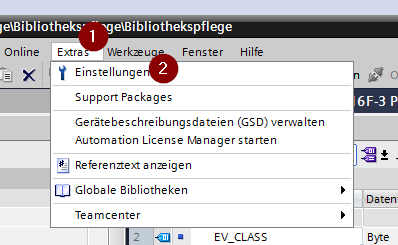
\includegraphics[width = 0.5 \textwidth]{Aufruf der Einstellungen.png}
    \caption{Aufruf der Einstellungen}
    \label{fig:Aufruf der Einstellungen}
\end{figure}

\begin{figure}[!ht]
    \centering
    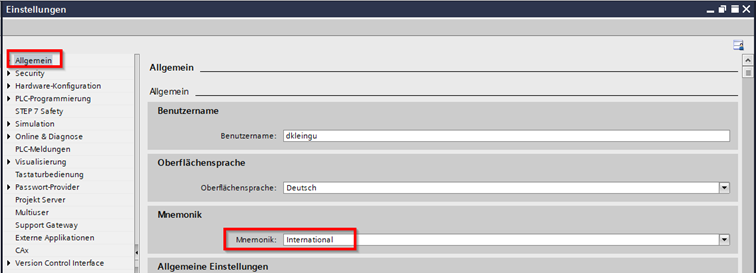
\includegraphics[width = 0.9 \textwidth]{Einstellung der Mnemonik.png}
    \caption{Einstellung der Mnemonik}
    \label{fig:Einstellung der Mnemonik}
\end{figure}

\clearpage
\section{Voreinstellung der Remanenz für nicht optimierte Bausteine}\label{subsec:Voreinstellung der Remanenz für nicht optimierte Bausteine}

Um Datenverlust nach CPU-Neustarts zu vermeiden, müssen die Datenbausteine mit dem Attribut \glqq Remanent \grqq{} deklariert werden. Diese Einstellung lässt sich per Voreinstellung standardmäßig aktivieren:

\begin{figure}[!ht]
    \centering
    \includegraphics[width = 0.7 \textwidth]{Voreinstellung der Remanenz für nicht optimierte Bausteine.png}
    \caption{Voreinstellung der Remanenz für nicht optimierte Bausteine}
    \label{fig:Voreinstellung der Remanenz für nicht optimierte Bausteine}
\end{figure}

\section{Einbindung globaler Bibliotheken in das TIA-Portal}\label{subsec:Einbindung globaler Bibliotheken in das TIA-Portal}
Der Speicherort für die Konfigurationsdatei zu Unternehmensbibliotheken befindet sich im TIA-Portal immer an der folgenden Stelle:\par
\noindent \textbf{TIA V14:} C:\textbackslash ProgramData\textbackslash Siemens\textbackslash Automation\textbackslash Portal V14\textbackslash CorporateSettings \par
\noindent
\noindent \textbf{TIA V15:} C:\textbackslash ProgramData\textbackslash Siemens\textbackslash Automation\textbackslash Portal V15\textbackslash CorporateSettings \par
\noindent
\noindent \textbf{TIA V17:} C:\textbackslash ProgramData\textbackslash Siemens\textbackslash Automation\textbackslash Portal V17\textbackslash CorporateSettings \par
\noindent
Um unsere vorhandenen Bibliotheken beim Start des TIA-Portals automatisch einzubinden, muss die Datei \glqq CorporateSettings.xml\grqq{} unter dem oben angegebenen Pfad (ACHTUNG: \glqq ProgramData\grqq{} ist ein versteckter Ordner) durch die passende Datei ersetzt werden. Je nachdem, wie ihr die Shared Folders in eurer VM eingestellt habt, kann es sein, dass ihr in der XML-Datei den Zielpfad an euer System anpassen müsst. Die benötigte Datei ist am folgenden Ort zu finden:\par 
\noindent \textbf{TIA V14:} I:\textbackslash Technik\textbackslash Software\textbackslash Bibliotheken\textbackslash TIA14\textbackslash CorporateSettings.xml \par
\noindent
\noindent \textbf{TIA V15:} I:\textbackslash Technik\textbackslash Software\textbackslash Bibliotheken\textbackslash TIA15\textbackslash CorporateSettings.xml \par
\noindent
\noindent \textbf{TIA V17 (VM):} I:\textbackslash Technik\textbackslash Software\textbackslash Bibliotheken\textbackslash TIA17\textbackslash CorporateSettings  \\ \textbackslash VM-Installation\textbackslash CorporateSettings.xml \par
\noindent
\noindent \textbf{TIA V17 (Host):} I:\textbackslash Technik\textbackslash Software\textbackslash Bibliotheken\textbackslash TIA17\textbackslash CorporateSettings \\ \textbackslash Host-Installation\textbackslash CorporateSettings.xml \par
\noindent


\clearpage
\subsection{Verfügbare Bibliotheken}\label{subsec:Verfügbare Bibliotheken}

\begin{longtable}{| p{\colwidth{0.4}} | p{\colwidth{0.6}} |} % columns widths have to add up to 1 otherwise there will be an over- or underfill of the table layout
    \hline
    \textbf{Name} & \textbf{Kommentar}\\    
    \hline
    Sample Library for Instructions & Beispielanwendungen von Siemens\\    
    \hline
    Buttons\_2Byte\_KREFELD & HMI-Button WinCC-Vorlage Krefeld\\    
    \hline
    LCon & Converting Toolbox von Siemens\\    
    \hline
    KeyPanelLibrary & Bausteine zur Ansteuerung der Key Panel der Firma Siemens\\    
    \hline
    LAcycCom & Bibliothek für azyklische Kommunikation mit S7-1x00\\    
    \hline
    LDrvSafe & Library Drive Safety, Bausteine zur Ansteuerung von G/S-Antrieben mit Profisafe\\    
    \hline
    LGF & Library of General Functions, Siemens, allgemeine nützliche Funktionen\\    
    \hline
    LPD & Library of PLC Datatypes, Datentypen zur einfachen Programmerstellung von Peripherie- und Technologiemodulen\\    
    \hline
    LLec & Lebbing-Bausteinbibliothek\\    
    \hline
    Sinamics\_telegram\_library & Bausteine + Datentypen zur Kommunikation mit S/G-Antrieben über Standardtelegramme\\    
    \hline
    
    \caption{Auflistung globaler Bibliotheken}\label{tab:Auflistung globaler Bibliotheken} %\label used for referencing the figure in text
\end{longtable}

\subsection{Aufruf der Bausteinhilfe}\label{subsec:Aufruf der Bausteinhilfe}

Um die Bausteinhilfe zu der Lebbing-Bausteinbibliothek aufzurufen, muss ein Baustein aus der Bibliothek markiert werden. Wird dann die Tastenkombination <SHIFT+F1> gedrückt, öffnet sich die Baustein-Hilfe im voreingestellten Standard-Browser. Dies funktioniert nur, so-lange man sich im internen Netzwerk der Fa. Lebbing befindet.
Soll die Bausteinhilfe auch außerhalb des Büros zur Verfügung stehen, müssen die Hilfedatei-en der Bibliothek manuell kopiert (am besten in den Projektordner) werden. Der zu kopierende Ordner lautet \glqq UserFiles\grqq{} und ist über den folgenden Pfad zu erreichen: I:\textbackslash Technik\textbackslash Software\textbackslash Bibliotheken\textbackslash TIA17\textbackslash LLec

\section{Weitere Einstellungen}\label{subsec:Weitere Einstellungen}
Weitere Einstellungen, z.B. das standardmäßige Einblenden der Variableninformationen, kann jeder Mitarbeiter seinen Vorlieben entsprechend anpassen.
